\documentclass[11pt]{article}
\usepackage[spanish]{babel}
\usepackage{amsmath}
\usepackage{amssymb}
\usepackage{graphicx}
\graphicspath{ {./images/}, {~/Apunte/images/} }
\usepackage[utf8]{inputenc}
\usepackage[T1]{fontenc}
\usepackage[margin=1in]{geometry}
\usepackage{fancyhdr}
\usepackage{hyperref}

\hypersetup{
    pdftitle={Tu Título},
    pdfauthor={Felipe Colli Olea},
    colorlinks=true,
    linkcolor=black,
    urlcolor=cyan
}

\pagestyle{fancy}
\fancyhf{}
\fancyfoot[C]{\footnotesize Felipe Colli, Todos los Derechos Reservados}
\fancyfoot[R]{\thepage}
\renewcommand{\headrulewidth}{0pt}

\title{Post Laboratorio 4}
\author{Felipe Colli}
\date{\today}

\begin{document}

\maketitle
\thispagestyle{fancy}

% ------------------------------------------------------------------------------
% INTRODUCCIÓN
% ------------------------------------------------------------------------------
\section{Introducción}

El presente informe detalla el trabajo realizado durante el cuarto laboratorio del curso, cuyo objetivo principal fue la introducción al análisis, procesamiento y visualización de datos numéricos mediante el uso de planillas de cálculo. A diferencia de las unidades anteriores enfocadas en la redacción estructurada (\LaTeX), esta etapa requirió un enfoque algorítmico y matemático para automatizar cálculos repetitivos.

Considerando la infraestructura de la facultad, el laboratorio fue desarrollado de manera presencial utilizando los equipos institucionales con sistema operativo Windows 11 y el software Microsoft Excel. Esto permitió aplicar de forma directa las lógicas operacionales, funciones integradas y sistemas de referenciación (absoluta y relativa) del ecosistema ofimático estándar exigido en la industria.

% ------------------------------------------------------------------------------
% DESARROLLO Y TRABAJOS REALIZADOS
% ------------------------------------------------------------------------------
\section{Desarrollo de Actividades}

El laboratorio se dividió en dos actividades principales orientadas a la evaluación de funciones matemáticas y la manipulación de datos multidimensionales a través de múltiples hojas de trabajo.

\subsection{Actividad 1: Análisis Numérico y Gráfico de una Función}
Se solicitó encontrar las raíces de un polinomio de cuarto grado donde un despeje analítico tradicional resultaba ineficiente. La función dada fue:
\begin{equation}
	f(x) = -\frac{x^4}{200} + \frac{x^3}{5} - 2x^2 + 50
\end{equation}

Para resolverlo, se implementó una tabulación en la planilla abarcando el intervalo de números enteros $x \in [-5, 25]$.
\begin{itemize}
	\item \textbf{Automatización:} El vector $x$ se construyó utilizando referencias relativas (ej. \texttt{=A2+1}). Posteriormente, la columna $f(x)$ fue programada traduciendo la notación algebraica a la sintaxis de Excel: \texttt{=-(A2*A2*A2*A2)/200 + (A2*A2*A2)/5 - 2*(A2*A2) + 50}.
	\item \textbf{Resultados:} Al graficar los pares ordenados $(x, f(x))$ mediante un gráfico de dispersión con líneas suavizadas, se identificaron los puntos donde la curva intercepta el eje de las abscisas ($f(x) = 0$). Se lograron visualizar claramente las raíces reales del polinomio numéricamente.
\end{itemize}

% Placeholder para la imagen de la Actividad 1
\begin{figure}[h]
	\centering
	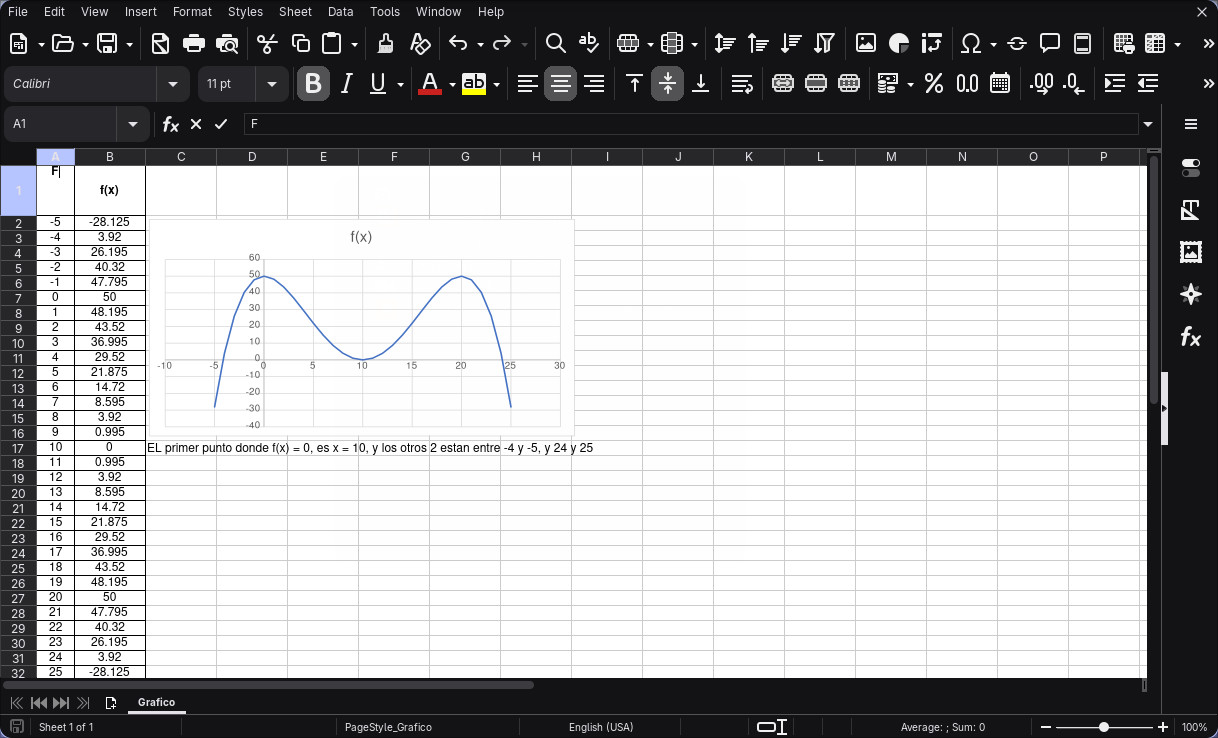
\includegraphics[width=0.8\textwidth]{excel1.png}
	\caption{Tabulación y gráfico de la función $f(x)$ (visualizado en Libre Office Calc en mi computador personal).}
\end{figure}

\subsection{Actividad 2: Conversión de Divisas y Referencias Cruzadas}
Esta actividad simuló un caso práctico de comparación comercial (el precio del libro \textit{El Marciano de Andy Weir}) evaluando su costo en diferentes monedas (EUR, GBP, JPY, USD, CLP).

\begin{itemize}
	\item \textbf{Manejo de Referencias:} Se crearon múltiples hojas para organizar la información de manera estructurada. Para calcular los valores en pesos chilenos (CLP), fue imperativo utilizar la sintaxis de \textbf{referencias entre hojas} (ej. \texttt{Hoja1!A1}) combinada de forma estricta con \textbf{referencias absolutas} (mediante el símbolo \texttt{\$}). Esto permitió fijar las tasas de conversión al arrastrar las fórmulas hacia celdas inferiores.
	\item \textbf{Funciones de Agregación y Visualización:} Una vez obtenida la tabla de precios estandarizada en CLP, se utilizaron las funciones estadísticas \texttt{=MAX()}, \texttt{=MIN()} y \texttt{=PROMEDIO()} para el análisis de los datos. Finalmente, se generó un gráfico de columnas que permitió una rápida comparación visual de los costos.
\end{itemize}

% Placeholder para la imagen de la Actividad 2
\begin{figure}[h]
	\centering
	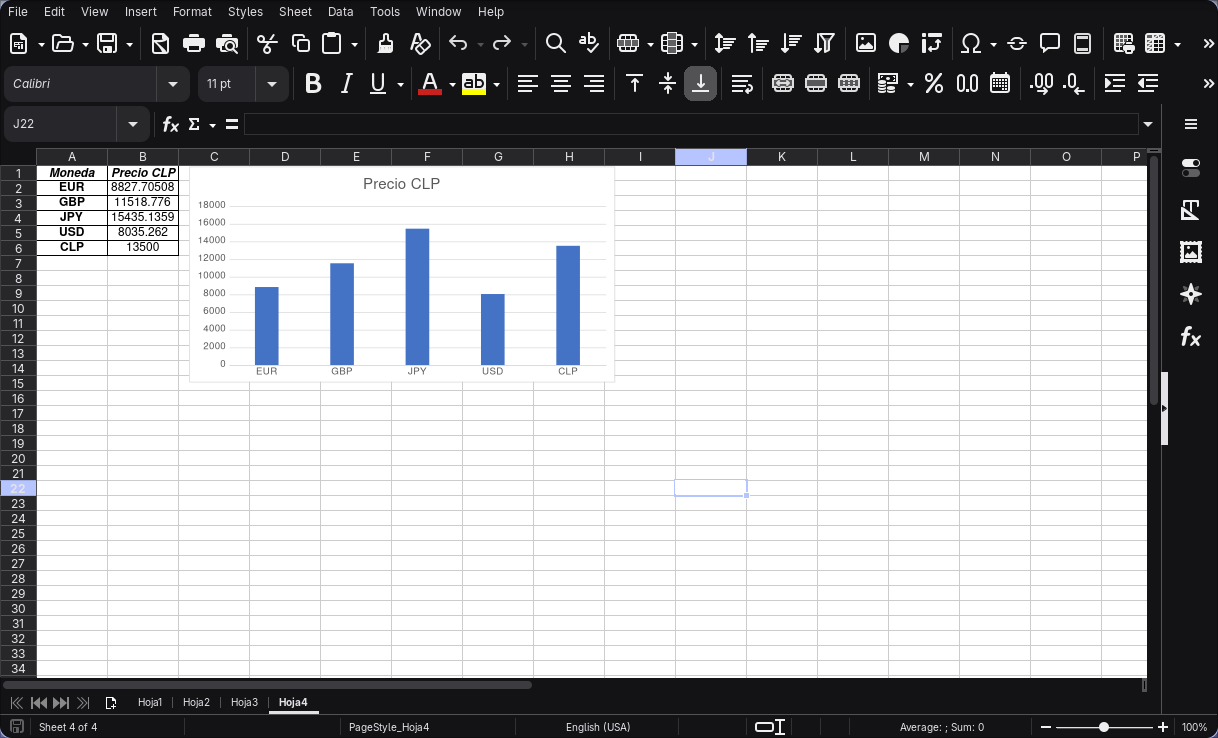
\includegraphics[width=0.8\textwidth]{excel2.png}
	\caption{Tabla de conversión monetaria y gráfico de columnas comparativo (visualizado en Libre Office Calc en mi computador personal).}
\end{figure}

\newpage
% ------------------------------------------------------------------------------
% REFLEXIONES Y DIFICULTADES
% ------------------------------------------------------------------------------
\section{Reflexiones y Dificultades}

A nivel técnico, la resolución del laboratorio no presentó desafíos matemáticos insalvables, pero sí supuso un desafío de adaptación en cuanto al flujo de trabajo. Acostumbrado a entornos de desarrollo basados enteramente en código y atajos de teclado (como \LaTeX{} o lenguajes de programación en Linux), la transición al entorno gráfico de Microsoft Excel en Windows requirió un cambio de paradigma.

La principal dificultad metodológica fue la extrema precaución visual que demanda la herramienta. En Excel, un error al arrastrar una fórmula sin haber fijado correctamente una celda con el símbolo \texttt{\$} produce un error de propagación silencioso. A diferencia de un compilador de código que arroja advertencias explícitas (\textit{warnings} o \textit{syntax errors}), la planilla asume que el usuario desea referencias relativas por defecto, lo que obliga a revisar meticulosamente la barra de fórmulas tras cada operación de autocompletado para evitar resultados matemáticamente incorrectos.

% ------------------------------------------------------------------------------
% CONCLUSIONES
% ------------------------------------------------------------------------------
\section{Conclusiones}

El Laboratorio 1 de Excel cumplió cabalmente su propósito de introducir los conceptos de referencias relativas, referencias absolutas, funciones estadísticas integradas y visualización gráfica de datos numéricos.

A través del desarrollo de las actividades, quedó demostrada la versatilidad de las planillas de cálculo como una herramienta de uso inmediato. Si bien carecen de la robustez estructural del código puro, su capacidad para realizar prototipos matemáticos de forma rápida (como encontrar las raíces de un polinomio complejo mediante tabulación) y generar reportes financieros visuales en cuestión de minutos, justifica plenamente por qué Microsoft Excel es un estándar transversal en el mundo de la ingeniería y la administración.

\end{document}
